\section*{Capítulo 01: Transaction Cost economics}

O autor destaca que o \textbf{objetivo} do livro é analisar as instituições do \textit{capitalismo} com especial ênfase às firmas, ao mercado e às relações contratuais e avança em direção de que as instituições têm o propósito de e efeito de reduzir os \textbf{custos de transação}. Na mesma seção, discute que o pouco conhecimento sobre as formas de organização decorre da relutância em reconhecer que as organizações importam. O estudo das instituições econômicas, no entanto, tem renascido de modo que a visão da firma enquanto uma função de produção vem sendo substituída pelo conceito de \textbf{estrutura de governança}. Em seguida, pontua que não se pode compreender a importância das instituições no capitalismo na ausência do conceito de \textbf{custos de transação} e esta abordagem pode ser caracterizada como:

\begin{itemize}
	\item Majoritariamente microanalítica
	\item Mais ciente das hipóteses comportamentais
	\item Introduz e avança no conceito de especificidade dos ativos
	\item Parte de uma análise institucional comparativa
	\item Trata as firmas enquanto uma estrutura de governança
	\item Dá maior ênfase as instituições contratuais \textit{ex post}
	\item Transação é a principal unidade de análise e reconhece que as organizações são relevantes
\end{itemize}

\subsection*{Custos de transação}

\paragraph*{Atrito}

Os custos de transação são o equivalente ao atrito em economia. Até a consideração deste conceito, outras formas de organização (não-padrão) eram pouco estudadas uma vez que a visão da firma enquanto uma função de produção prevalecia.

\paragraph*{Explicação}

Economia dos custos de transação (ECT) trata o problema da organização econômica enquanto um problema \textbf{contratual}. Neste ponto, cabe distinguir custos de transação em \textit{ex ante} e \textit{ex post}. O primeiro diz respeito aos custos de elaboração, negociação e estabelecimento de salvaguardas de um contrato. Parte significativa dos estudos parte da hipótese de que os custos e implementação do sistema jurídico são eficientes. Como consequência, verifica-se a divisão entre economistas e juristas em que os primeiros se especializam na troca e os segundos nos contratos. Os contratos \textit{ex post}, por sua vez, possuem diferentes formas:
	(1) custos mal adaptados em relação a desvios na curva de contratos;
	(2) custos de negociação se os esforços bilaterais são feitos de modo a corrigir os desacordos \textit{ex post};
	(3) custos de configuração e execução das estruturas de governança aos quais as disputas (não judiciais) se referem e;
	(4) custos de efetivação de acordos seguros.
De todo modo, os contratos \textit{ex ante} e \textit{ex post} devem ser analisados \textbf{simultaneamente} e não sequencialmente. Além disso, como os custos de transação são analisados \textbf{comparativamente}, é a diferença relativa entre as estruturas organizacionais que são mais relevantes.

\paragraph*{Contexto mais amplo}

Aspectos importantes dos custos de transação:

\begin{itemize}
	\item A economia dos custos se refere à somo dos custos de produção e de transação e os respectivos \textit{trade-offs} entre ambos devem ser identificados
	\item O tipo de bem e serviço ofertado é uma \textbf{variável de decisão} que influencia tanto a demanda quanto os custos de transformação e transação
	\item O contexto social é relevante
	\item Sempre que os custos privados e coletivos se diferem, os custos sociais dominar se forem tentados acordos prescritivos
\end{itemize}


\subsection*{Mapa teórico-cognitivo dos contratos}

Ao longo desta seção, o autor faz referência ao mapa abaixo:

\begin{figure}[H]
	\centering
	\caption{Mapa cognitivo dos contratos}
	\label{fig:screenshot001}
	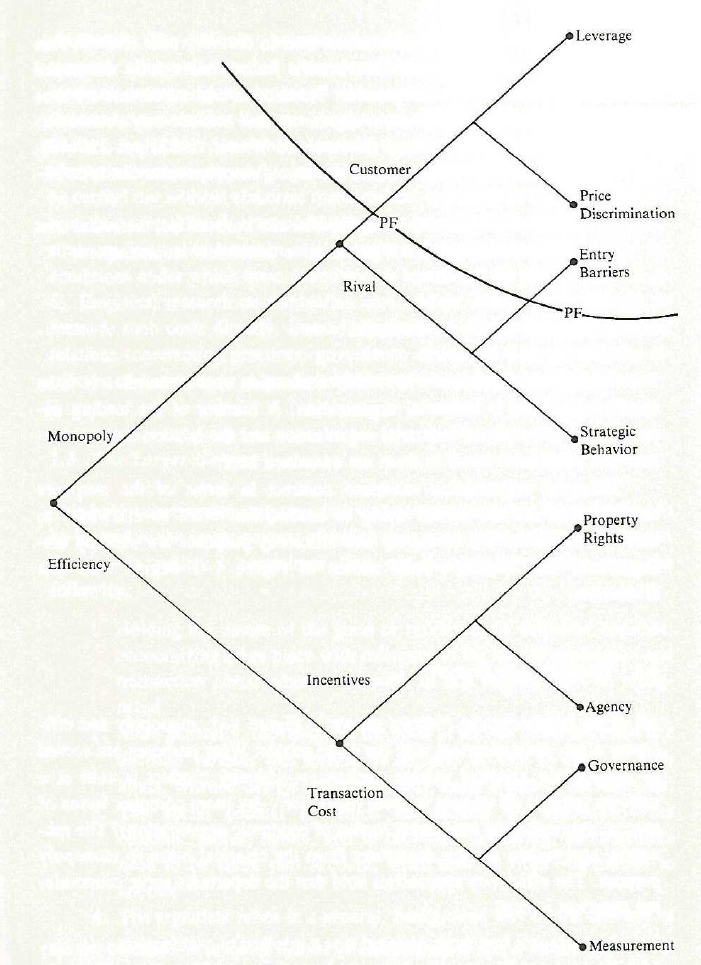
\includegraphics[width=0.7\linewidth]{screenshot001}
\end{figure}

Por mais que este esquema evidencie diversos ramos, são analisados os que dizem respeito à ECT ao longo desta resenha.
No ramo da eficiência e subramificação dos \textbf{incentivos}, tanto a literatura dos direitos de propriedade quanto de agência consideram que os problemas contratuais são resolvidos \textit{ex ante} e que o sistema jurídico é eficiente. Diferentemente do ramo ``Monopólio'' e similarmente à ECT, o ramo dos incentivos consideram que formas não convencionais de organização têm por objetivo a eficiência. No que diz respeito à ETC, em particular, maior atenção é dada na \textbf{execução} do contrato e menos na elaboração. Também em consonância com a literatura de direitos de propriedade, a ETC reconhece que a delimitação da propriedade é relevante, mas dando especial ênfase determinação \textbf{privada}. Em outras palavras, a ECT adiciona a proposição de que instituições \textit{ex post} importam.

No ramo da ECT, Williamson destaca a literatura de governança e de mensuração dos custos de transação. O objetivo da primeira não é apenas resolver conflitos em andamento, mas detectar conflitos potenciais e recomendar estruturas de governança para evitá-los. O segundo ramo, por sua vez, está mais preocupado com a performance associada à oferta de bens e serviços.


\subsection*{Mundo do contrato}

Esta seção discute os diferentes tipos de contratos associados às hipóteses comportamentais e reconhecimento (ou não) da especificidade dos ativos tal como ilustrado na tabela seguinte:

\begin{figure}[H]
	\centering
	\caption{Atributos do processo contratual}
	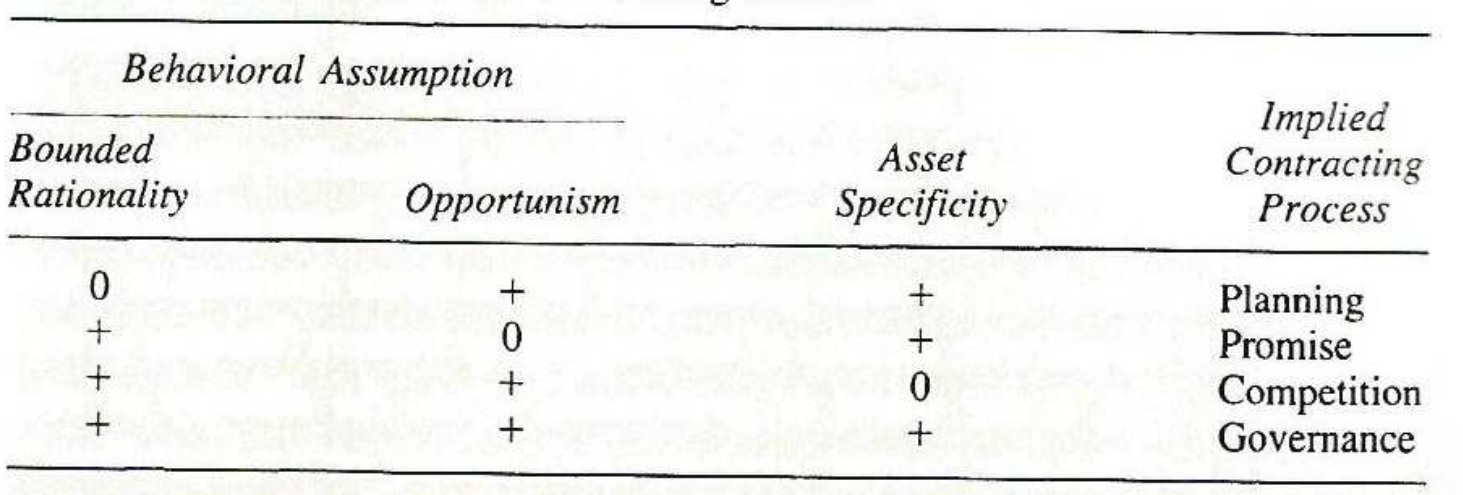
\includegraphics[width=0.7\linewidth]{screenshot002}
	\label{fig:screenshot002}
\end{figure}
Tal como feito anteriormente, será dada maior ênfase às contribuições da ECT.
Em linhas gerais, as outas formas de contrato (planejamento, promessa e competição) falham na presença de \textbf{racionalidade limitada}, \textbf{comportamento oportunista} e \textbf{especificidade dos ativos}. Este é o mundo ao qual a ECT se debruça. Mais detalhadamente, planejamento é incompleto por conta da racionalidade limitada; promessa não é cumprida por conta da existência do comportamento oportunista e; a competição não-identificada não é satisfatória por conta da especificidade dos ativos.

\subsection*{Esquema simples de contrato}

Williamson apresenta um esquema que ilustra diferentes formas de contrato considerando ausência ($k=0$) ou presença de ativos específicos ($k>0$) e de salvaguardas. Neste esquema, $A$ refere-se a uma tecnologia sem ativos específicos e sem salvaguardas, $B$ apresenta apenas especificidades de ativos e $C$ possui tanto ativos específicos quanto salvaguardas. A partir deste esquema, é possível analisar questões contratuais de forma comparativa em termos da tecnologia ($k$), governança contratual ($s$) e determinação de preços ($p$) de forma simultânea. Em seguida, apresenta as propriedades deste esquema:

\begin{figure}
	\centering
	\caption{Esquema simples de contrato}
	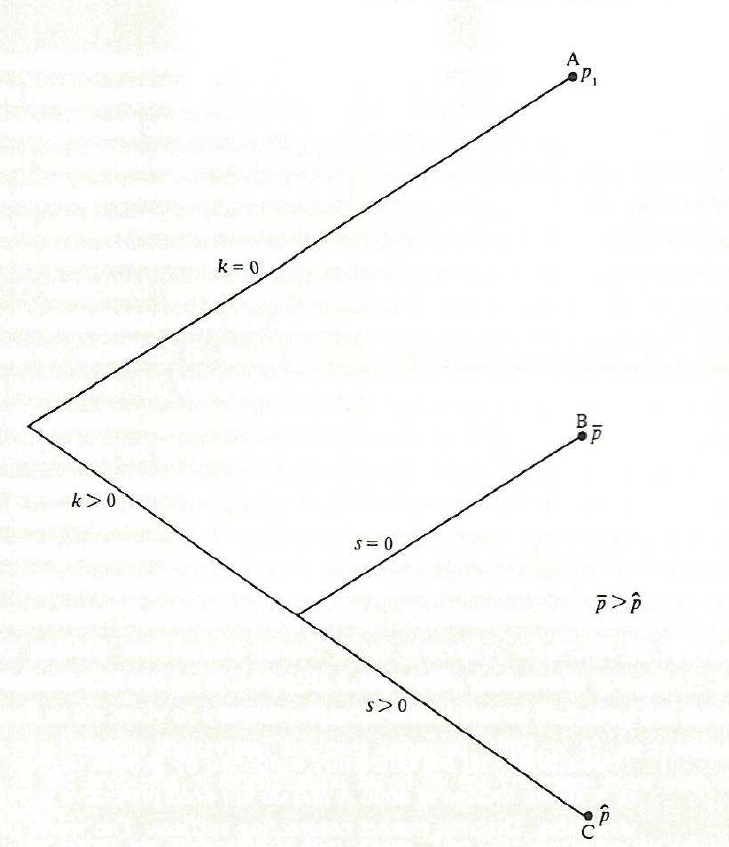
\includegraphics[width=0.7\linewidth]{screenshot003}
	\label{fig:screenshot003}
\end{figure}

\begin{itemize}
	\item Uma transação geral, sem especificidade de ativos, não requer uma estrutura de governança específica para ser eficiente;
	\item Transações com especificidade de ativos são aquelas que são eficientemente alocadas em uma transação bilateral
	\item Uma transação como a $B$ não é sustentável
\end{itemize}

\subsection*{Ortanização econômica da \textit{Company town}}

Por se tratar de um estudo de caso, não será analisada nesta resenha.

\subsection*{Aplicações}

Os temas microeconômicos passíveis de ser analisados de acordo com a ECT são os seguintes:
\begin{itemize}
	\item Restrições de marcados verticais
	\item Discriminação de preços
	\item Regulação
\end{itemize}

\subsection*{Conclusões}

As proposições da ECT são as seguintes:
\begin{itemize}
	\item A transação é a unidade básica de análise
	\item Qualquer problema econômico pode ser traduzido (direta e indiretamente) em termos de um problema contratual e enfatizar os custos de transação
	\item Designa os tipos de transação às estruturas de governança de acordo com
	\begin{itemize}
		\item Atributos das transações
		\item Incentivos e atributos adaptativos de estruturas de governança alternativas
	\end{itemize}
	\item Prioriza uma análise comparativa das distintas formas institucionais
	\item Qualquer tentativa de analisar as organizações econômicas deveria considerar racionalidade limitada e comportamento oportunista conjuntamente com especificidade dos ativos
\end{itemize}
Apresentados as propostas centrais da ECT, Williamson destaca a \textbf{especificidade dos ativos} enquanto elemento distintivo entre as diferentes formas de governança.